\documentclass{article}
\usepackage{graphicx}
\usepackage{amsmath}
\usepackage{amsfonts} 
% or 
\usepackage{amssymb}

\usepackage{tikz}
\usepackage{pgfplots}
\usepgfplotslibrary{fillbetween}
\usetikzlibrary{patterns}

\pgfplotsset{compat = newest}
\usepackage{cancel}
\usepackage[margin=1in]{geometry}

\begin{document}

\title{A-Level Maths Notes}
\maketitle

\section{Laws of Indices}

\subsection{Subsets of Real Numbers}

\subsubsection{Natural Numbers}
Natural Numbers are positive whole numbers. Weather or not Zero is natural
is disputed but the exam boards say it isn't. They are the "Counting Numbers"
 and are represented by the following:

\begin{equation}
    \label{simple_equation}
    \mathbb{N}_0 = \{0, 1, 2, \dots\}
\end{equation}

\begin{equation}
	\label{simple_equation}
    \mathbb{N}_1 = \{1, 2, 3, \dots\}
\end{equation}

\subsubsection{Integers}
Integers are whole numbers. They can be positive or negative  and are represented by the following:

\begin{equation}
    \label{simple_equation}
    \mathbb{Z} = \{\dots, -3, -2, -1, 0, 1, 2, 3, \dots\}
\end{equation}

\subsubsection{Rational Numbers}
Rational Numbers are any real number that can be represented by a fraction. They are represented by the following:

\begin{equation}
	\label{simple_equation}
	\mathbb{Q} = \{ x | x = \frac{a}{b}, a,b \in \mathbb{Z} \text{ and } b \ne 0 \}
\end{equation}

\subsubsection{Real Numbers}
A real number is any number that is not complex or imaginary. They are represented by the following:

\begin{equation}
	\label{simple_equation}
	\mathbb{R} = \{x | -\infty <  x <\infty\}
\end{equation}

\begin{equation}
	\label{simple_equation}
	\mathbb{N} \subset \mathbb{Z} \subset \mathbb{Q} \subset \mathbb{R}
\end{equation}

\break
\subsection{Indices: The Laws of Indices}

\subsection{Multiplying Indices}
When multiplying indicies the following is true:
\begin{equation}
	\label{simple_equation}
	x^{p} \times x^{q} = x^{p + q}
\end{equation}
This reason for this becomes clear when we expand the expressions.
\\
For example:
\begin{gather*}
	x^2 \times x^3 = x^5\\
	\underbrace{
		\overbrace{x \times x}^{x^2} \times
		\overbrace{x \times x \times x}^{x^3}
	}_{x^5}
\end{gather*}

\subsubsection{Powers of Indices}

\begin{equation}
	\label{simple_equation}
	x^{pq} = (x^{p})^{q} = (x^{q})^{p} 
\end{equation}
The reason for this becomes clear when we expand the expressions.
\\
For example:

\begin{gather*}
	(x^2)^3 = x^6\\
	\underbrace{
		\overbrace{x \times x}^{x^2} \times
		\overbrace{x \times x}^{x^2} \times
		\overbrace{x \times x}^{x^2}
	}_{x^6}
\end{gather*}
\subsubsection{Division}

\begin{equation}
	\label{simple_equation}
	x^{p - q} = \frac{x^{p}}{x^{q}}
\end{equation}
The reason for this becomes clear when we expand the expressions.
\\
For example:

\begin{gather*}
	\frac{x^3}{x^2} = x^1\\
	\frac{\overbrace{x \times x \times x}^{x^3}}{\underbrace{x \times x}_{x^2}} =
	\frac{\overbrace{\cancel{x} \times \cancel{x} \times x}^{x^3}}{\underbrace{\cancel{x} \times \cancel{x}}_{x^2}} =
	x
\end{gather*}
\subsubsection{Rational Exponents}
Any rational exponent can be expressed as a power and a root:
\begin{equation}
	\label{simple_equation}
	\sqrt[q]{x}^{p} = x^{\frac{p}{q}}
\end{equation}


\begin{equation}
	\label{simple_equation}
	\sqrt[p]{x} = x^{\frac{1}{p}}
\end{equation}

\subsubsection{Zero}
Anything with a power of $0$ is always $1$ even in the case of $0$.
\begin{equation}
	\label{simple_equation}
	x^0 = 1
\end{equation}
This is true because you can always add a $\times 1$ as shown below:
\begin{equation}
	x^0 = 1 \times x^0 = 1 \times \cancel{x^0} = 1
\end{equation}

\subsubsection{Negative Exponents}
Negative exponents are defined as the following, this means that a larger magnitude of $p$ when $x>1$
will result in the expression evaluating to a smaller number.
\begin{equation}
	\label{simple_equation}
	x^{-p} = \frac{1}{x^p}
\end{equation}

\subsubsection{Reciprical}
The reciprocal is a special case of a negative exponent where the exponent is always $-1$.
\begin{equation}
	\label{simple_equation}
	x^{-1} = \frac{1}{x}
\end{equation}

\break
\section{Quadratic Functions and Graphs}

\subsection{Factorising Quadratics}

\subsubsection{Difference of Two Squares}
The difference of two squares is a rule that can help us
factorise quadratics in the form $ax^2 + b$ by using the
following identity:

\begin{equation}
	(a - b)(a + b) = a^2 + b^2
\end{equation}
The proof of this is fairly straight forward; we simply expand and simplify $(a - b)(a + b)$ to get $a^2 + b^2$.
\\
We can apply this identity when given a quadratic in the form $ax^2 + c$.

\begin{align*}
	&\text{First we rearrange to fit the identity}\\
	&(x\sqrt{a})^2 + \sqrt{c}^2\\
	&\text{Then we use the identity to split the expression into factors}\\
	&(x\sqrt{a} - \sqrt{c})(x\sqrt{a} + \sqrt{c})
\end{align*}
For example, we can factorise the quadratic $25x^2 - 16$:

\begin{align*}
	&\text{First we rearrange to fit the identity}\\
	&(x\sqrt{25})^2 - \sqrt{16}^2 = (5x)^2 - 4^2\\
	&\text{Then we use the identity to split the expression into factors}\\
	&(5x - 4)(5x + 4)
\end{align*}

\subsubsection{Factorising Quadratics in the form $x^2 + bx + c$}
In order to factorise a quadratic in the form $x^2 + bx + c$,
we need to find two numbers, $e$ and $f$ where $e + f = b$ and
$e \times f = c$ then sub them into the following expression:
\begin{equation}
	(x + e)(x + f)
\end{equation}
\\
For example, if given the quadratic $x^2 + 5x + 6$ we can factorise as shown by the following:
\begin{align*}
	2 \times 3 &= 6 \\
	2 + 3 &= 5 \\
	&\therefore \\
	x^2 + 5x + 6 &= (x + 2)(x + 3)
\end{align*}

\subsubsection{Factorising Quadratics in the form $ax^2 + bx + c$}
In order to factorise a quadratic in the form $ax^2 + bx +c$, we must first factor out $a$.
This gives us the following expression:
\begin{equation}
	a\left(x^2 + \frac{bx}{a} + \frac{c}{a} \right)
\end{equation}
\\
This makes it easy to factorise quadratics where both $b$ and $c$ are divisible by $a$
For Example, we can factorise the expression $2x^2 + 10x + 12$ with the following steps:

\begin{gather*}
	\text{We start by factoring out a}\\
	2\left(x^2 + \frac{10x}{2} + \frac{12}{2} \right) = 2(x^2 + 5x + 6)\\
	\text{We then factorise the new quadratic}\\
	2((x+2)(x+3)) = 2(x+2)(x+3)\\
	\text{Often our answer will be required in the form $(x + a)(x + b)$}\\
	(2x + 4)(x + 3) \text{ or } (x + 2)(2x + 6)
\end{gather*}
\\
However in some casees neither $b$ or $c$ are divisible by $a$.
For Example $16x^2 - 8x - 3$ though we can still use the same method.

\begin{gather*}
	16\left(x^2 - \frac{8}{16} - \frac{3}{16}\right)\\
	16\left(x + \frac{3}{4}\right)\left(x - \frac{1}{4}\right)
\end{gather*}
\subsection{Completing the Square}
Completing the square is act of rearranging a quadratic into the form $a(x + b)^2 +c$ to tell
us more information about the quadratic such as the turning point.

\subsubsection{Completing the Square for Quadratics in the form $x^2 + bx + c$}
For quadratics with a unit $x^2$ coefficient, we write our answer in the form \\
$(x+b)^2 + c$. To do this we use the steps show in the following example:
\\\\
We start with a quadratic:
\begin{equation}
	x^2 + 8x + 20
\end{equation}
We then half then make an expression in the form $(x+a)^2$ that
is equivalent to the same first two terms as the quadratic we started with
We do this by halving $b$ and putting it inside the brackets like so
\begin{equation}
	(x+4)^2 - 16= x^2 + 8x
\end{equation}
We then add a value on the end to make the starting quadratic
and the expression we ended up with equivalent
\begin{equation}
	(x + 4)^2 - 16 + 20 (x + 4)^2 - 16 + 20 
\end{equation}

\subsubsection{Completing the Square for Quadratics in the form $ax^2 + bx + c$}
For quadratics in with an $x^2$ coefficient that is not equal to $1$ it gets slightly more
complicated but the core idea stays the same.
\\\\
We start with a quadratic:
\begin{equation}
	2x^2 + 8x + 3
\end{equation}
We then factor out the $x^2$ coefficient like so:
\begin{equation}
	2(x^2 + 4x) + 3
\end{equation}
We then use the same method as previous this time remembering to multiply the number we move out of the parenthesis by $2$:
\begin{equation}	
	2(x + 2)^2 - 8 + 3 = 2(x + 2)^2 - 5
\end{equation}
\pagebreak
\subsection{Parabolas}

\subsubsection{Plotting Parabolas}
One way of plotting parabolas is to work out some specific points on the parabola and plot them.
\\
To do this we first start by calculating the y values for a given set of x values as shown below for
$y = x^2$:
\begin{center}
	\begin{tabular}{ | c | r | r | r | c | c | c | c | }
		\hline
		$x$ & $-3$ & $-2$ & $-1$ & $0$ & $1$ & $2$ & $3$\\ \hline
		$y=x^2$ &$9$ & $4$ & $1$ & $0$ & $1$ & $4$ & $9$\\
		\hline
	\end{tabular}
\end{center}
Once we have this data we can then plot it onto a graph such as the one below:
\begin{center}
	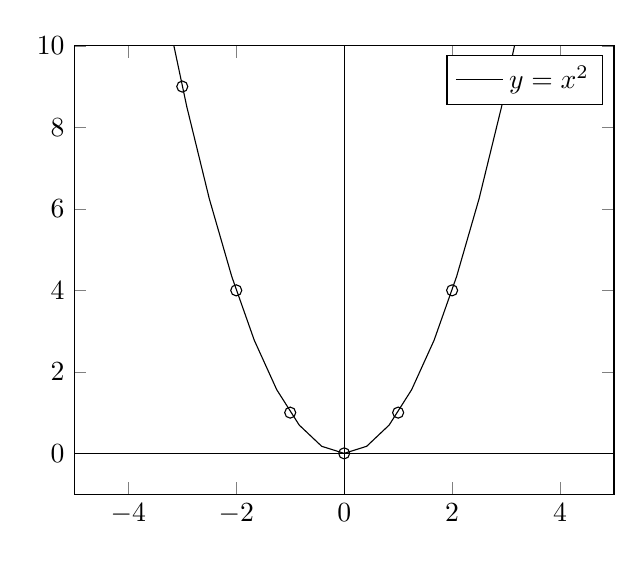
\begin{tikzpicture}
		\begin{axis}[
			xmin=-5, xmax=5,
    		ymin=-1, ymax=10,
		]
			\addplot[] {x^2};
			\addplot[only marks,mark=o] coordinates{(-3,9) (-2,4) (-1,1) (0,0) (1,1) (2,4) (3,9)};
			\legend{$y=x^2$}
			\draw[-] (-5,0)--(5,0);
			\draw[-] (0,-1)--(0,10);
		\end{axis}
	\end{tikzpicture}
\end{center}
\subsubsection{Sketching Parabolas from factorised quadratics}
In order to sketch a parabola, we need to know 3 points: Where on the parabola $x=0$ and 
where on the parabola $y=0$. We can do this by factorising. For example, the quadratic
$x^2 - x - 2$ can be factorised into $(x+1)(x-2)$. From there we can calculate the roots as
$(-1, 0)$ and $(2, 0)$ and the y intercept as $(0, -2)$. We can then roughly mark them on
some axis and then sketch a parabola that passes through those points.

\begin{center}
	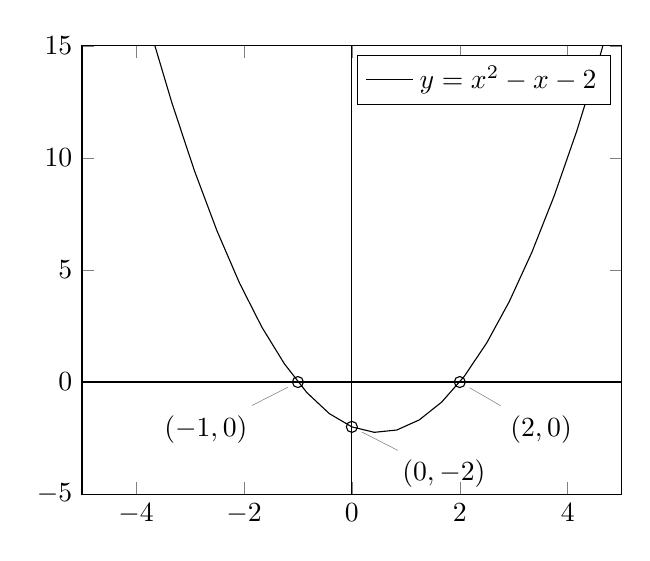
\begin{tikzpicture}
		\begin{axis}[
			xmin=-5, xmax=5,
    		ymin=-5, ymax=15,
		]
			\addplot[] {x^2 - x - 2};
			\addplot[only marks,mark=o] coordinates{(0,-2)} node[pin=-30:{$(0,-2)$}]{};
			\addplot[only marks,mark=o] coordinates{(-1,0)} node[pin=-150:{$(-1,0)$}]{};
			\addplot[only marks,mark=o] coordinates{(2,0)} node[pin=-30:{$(2,0)$}]{};
			\legend{$y=x^2 - x - 2$}
			\draw[-] (-8,0)--(8,0);
			\draw[-] (0,-25)--(0,15);		\end{axis}
	\end{tikzpicture}
\end{center}
\subsubsection{Sketching Parabolas from Completed Square Form}
To sketch a parabola from the completed square form we need to find 2 points: the y intercept (where $x=0$) and the turning point
(where $y$ is at its lowest value).
\\
Given a quadratic in the form $a(x+b)^2+c$ the turning point can be expressed as $(-b, c)$. This works because changing the
value of $b$ translates the graph on the $x$ axis and changing the value of $c$ translates the graph on the $y$ axis as show
below.
\\
For example, given the quadratic $(x + 2)^2 + 1$, the turning point is $(-3, 4)$ as shown on the graph below:

\begin{center}
	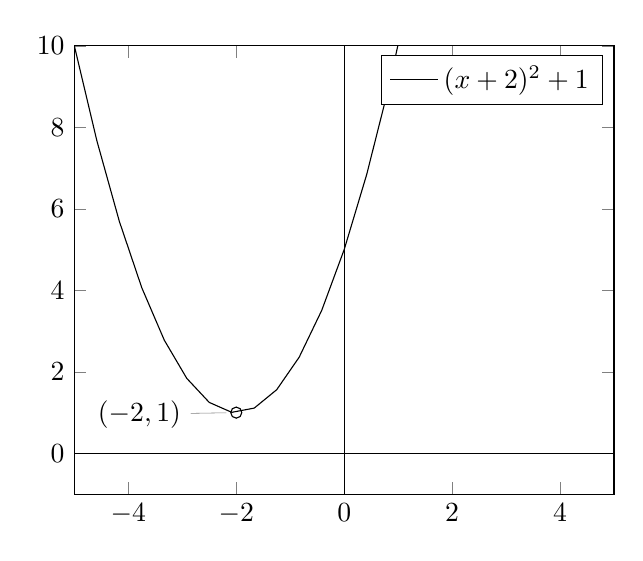
\begin{tikzpicture}
		\begin{axis}[
			xmin=-5, xmax=5,
    		ymin=-1, ymax=10,
		]
			\addplot[] {(x + 2)^2 + 1};
			\addplot[only marks,mark=o] coordinates{(-2,1)} node[pin=182:{$(-2,1)$}]{};
			\legend{$(x + 2)^2 + 1$}
			\draw[-] (-8,0)--(8,0);
			\draw[-] (0,-25)--(0,15);
		\end{axis}
	\end{tikzpicture}
\end{center}
To finish our sketch we need to find the $y$ intercept. To start we just replace $x$ with $0$ as were looking for the
point where $x=0$.
\\
For our previous example it would be as follows:

\begin{equation}
	y = (0 + 2)^2 + 1
\end{equation}
We then evaluate the right hand side of the equation to get our $y$ value:
\begin{equation}
	y = (0 + 2)^2 + 1 = (2)^2 + 1 = 4 + 1 = 5
\end{equation}
We can then use this information to plot our y intercept, $(0, 5)$, so we can sketch our graph.

\begin{center}
	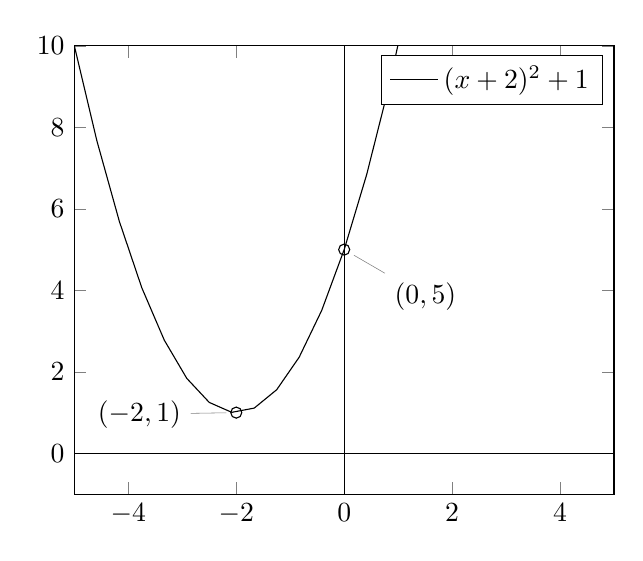
\begin{tikzpicture}
		\begin{axis}[
			xmin=-5, xmax=5,
    		ymin=-1, ymax=10,
		]
			\addplot[] {(x + 2)^2 + 1};
			\addplot[only marks,mark=o] coordinates{(-2,1)} node[pin=182:{$(-2,1)$}]{};
			\addplot[only marks,mark=o] coordinates{(0,5)} node[pin=-30:{$(0,5)$}]{};
			\legend{$(x + 2)^2 + 1$}
			\draw[-] (-8,0)--(8,0);
			\draw[-] (0,-25)--(0,15);
		\end{axis}
	\end{tikzpicture}
\end{center}
\break
\section{Surds}
Surds are the combination of a coefficient and a root in the form $a\sqrt{b}$ that can be used to 
represent a subset of irrational numbers.

\subsection{Rules of Surds}
The product of two surds is equal to a single surd with a base equal to the product of the two starting bases and
a coefficient equal to the product of the two starting coefficients. This can be written as follows:

\begin{equation}
	a\sqrt{b} \times c\sqrt{d} = ac\sqrt{bd}
\end{equation}

\subsection{Simplifying Surds}

Inorder to simplify surds we use the surd product rule shown previously. We break apart a single surd into two surds,
one where the base is square and then simplify as shown in the following example:

\begin{align*}
	&\text{We start by splitting the surd into two}\\
	&\sqrt{200} = \sqrt{25} \times \sqrt{8}\\
	&\text{Then, since $25$ is square, we can simplify} \\
	&\sqrt{200} = 5\sqrt{8}
\end{align*}
This also works if the starting surd has a coefficient:


\begin{align*}
	&\text{We start by splitting the surd into two}\\
	&2\sqrt{200} = 2 \times \sqrt{25} \times \sqrt{8}\\
	&\text{Then, since $25$ is square, we can simplify} \\
	&2\sqrt{200} = 10\sqrt{8}
\end{align*}
\subsection{Adding and subtracting surds}
Adding and subtracting surds is a bit like adding and subtracting fractions so it's important to remember the following:
\begin{equation}
	\sqrt{a} + \sqrt{b} \ne \sqrt{a + b}
\end{equation}
Instead the following is true:
\begin{equation}
	a\sqrt{c} + b\sqrt{c} = (a + b)\sqrt{c}
\end{equation}
This means that, to add and subtract surds, the base numbers must be equal. So we must, using previous rules,
put them into the form $a\sqrt{c} + b\sqrt{c}$ as shown in the following worked example:


\begin{align*}
	\sqrt{20} + \sqrt{180} &= \sqrt{4} \times \sqrt{5} + \sqrt{36} \times \sqrt{5}\\
	\sqrt{20} + \sqrt{180} &= 2\sqrt{5} + 6\sqrt{5} = 8\sqrt{5}
\end{align*}
\break
\subsection{Rationalising the Denominator}
Rationalising the denominator is the process of manipulating a fraction to make its denominator a rational number.
This often has the side affect of making the neumerator irrational.
\\
For simple fractions we can simply multiply by the surd in the denominator.
\begin{equation}
	\frac{a}{\sqrt{b}}=\frac{a \times \sqrt{b}}{\sqrt{b} \times \sqrt{b}}=\frac{a\sqrt{b}}{b}
\end{equation}
\\
For denominators with 2 or more terms this becomes more difficult and so you can't do the same thing.
\\
\begin{equation}
	\frac{a}{b + \sqrt{c}}=\frac{a \times \sqrt{c}}{(b + \sqrt{c}) \times \sqrt{c}}=\frac{a\sqrt{c}}{b\sqrt{c} + c}
\end{equation}
\\
Instead we multiply by $b - \sqrt{c}$ which gives us a rational denominator of $b^2 -c$ as show by the table below:

\begin{center}
	\begin{tabular}{ c | c | c }
		$\times$ & $b$ & $-\sqrt{c}$ \\ \hline
		$b$ & $b^2$ & $-b\sqrt{c}$ \\ \hline
		$\sqrt{c}$ & $b\sqrt{c}$ & $-c$
	\end{tabular}
\end{center}
We use this to give us the final fraction with a rational denominator as shown below:

\begin{equation}
	\frac{a}{b + \sqrt{c}}=\frac{a \times (b - \sqrt{c})}{(b + \sqrt{c}) \times (b - \sqrt{c})}=\frac{ab-a\sqrt{c}}{b^2 - c}
\end{equation}

\break
\section{Simultaneous Equations}
Simultaneous equations are sets of equations whos variables have the same values.
For example, the following are simultaneous equations:
\begin{align*}
	3x + y &= 5 \\
	4x - y &= 2
\end{align*}

\subsection{Elimination Method}
The elimination method is one method of solving simultaneous equations. This involves either adding or subtracting
equations from eachother in an attempt to cancel one of the terms. For example, we can solve the following using this
method:
\begin{align*}
	3x + y &= 5 \\
	4x - y &= 2 \\
	(3x + y) + (4x - y) &= 5 + 2\\
	7x &= 7\\
	x &= 1
\end{align*}
We can then solve the last bit of our equation by substituting in the value we found as follows:
\begin{align*}
	3x + y &= 5 \\
	3(1) + y &= 5 \\
	3 + y &= 5\\
	y &= 2\\
\end{align*}
This can become slightly more tricky for cases such as the following:
\begin{align*}
	3x + 2y &= 6 \\
	4x - y &= 9
\end{align*}
To solve this one we can multiply everything in one of the equations by 2 and then procede as normal:

\begin{align*}
	3x + 2y &= 6 \\
	4x - y &= 9 \\
	8x - 2y &= 18 \\
	(3x + 2y) + (8x -2y) &= 6 + 18 \\
	11x &= 24 \\
	&\vdots
\end{align*}

\break
\subsection{Substitution Method}
The substitution method is another, slightly more intuitive method of solving simultaneous equations. We start by rearranging
one of the equations to leave a single variable on it's own and then substitute that into the other equation. For example, we
can do the following to solve our first example:
\begin{align*}
	3x + y &= 5 \\
	4x - y &= 2 \\
	y &= 5 - 3x \\
	4x - (5 - 3x) &= 2 \\
	4x - 5 + 3x &= 2 \\
	7x - 5 &= 2 \\
	7x &= 7 \\
	x &= 1 \\
\end{align*}
We can then substitute $x$ to get our value for $y$ as shown in the following:
\begin{align*}
	3x + y &= 5 \\
	3(1) + y &= 5 \\
	3 + y &= 5\\
	y &= 2\\
\end{align*}
Unlike the previous method, we do not need to do anything special when there are no common coefficients in the equations.

\begin{align*}
	3x + 2y &= 6 \\
	4x - y &= 9 \\
	4x - 9 &= y \\
	3x + 2(4x - 9) &= 6 \\
	3x + 8x - 18 &= 6 \\
	11x - 18 &= 6 \\
	11x &= 24\\
	&\vdots
\end{align*}

\break

\subsection{Simultaneous Equations with Quadratics}
This even works when the equations are quadratic such as the following example:
\begin{align*}
	y &= 2x + 5\\
	y &= x^2 + 3x + 5 \\
	2x + 5 &= x^2 + 3x + 5 \\
	0 &= x^2 + x \\
	0 &= x(x + 1)\\
	x &= 0 \\
	x &= -1
\end{align*}
We then substitute the two values of $x$ to get the two $y$ values as follows:
\begin{align*}
	y &= 2x +5 \\
	y &= 2(0) + 5\\
	y &= 5 \\
	y &= 2(-1) + 5\\
	y &= 3
\end{align*}
This means that the two equations intersect at the points $(0, 5)$ and $(-1, 3)$ as shown on the axis below:

\begin{center}
	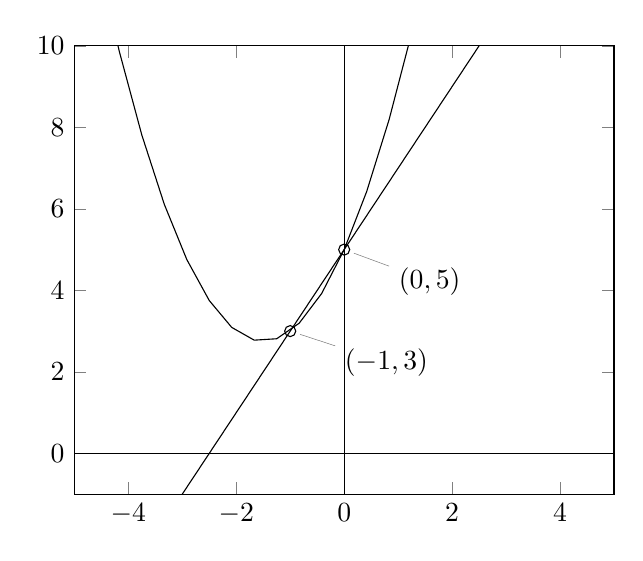
\begin{tikzpicture}
		\begin{axis}[
			xmin=-5, xmax=5,
    		ymin=-1, ymax=10,
		]
			
			\addplot[] {2 * x + 5};
			\addplot[] {x^2 + 3 * x + 5};
			\addplot[only marks,mark=o] coordinates{(-1,3)} node[pin=-10:{$(-1,3)$}]{};
			\addplot[only marks,mark=o] coordinates{(0,5)} node[pin=-10:{$(0,5)$}]{};
			\draw[-] (-8,0)--(8,0);
			\draw[-] (0,-25)--(0,15);
		\end{axis}
	\end{tikzpicture}
\end{center}

\section{Inequalities}
Inequalities are equations that use relation operators such as $<$, $>$, $\leq$ or $\geq$ instead of $=$.
\subsection{Simple Linear Inequalities}
For simple, linear inequalities we can solve them just like any other equation. For example:
\begin{equation}
	6x < 12 \Rightarrow x < 2
\end{equation}
Or for a slightly more complicated example:
\begin{equation}
	4 + 7x \leq 18 \Rightarrow 7x \leq 14 \Rightarrow x \leq 2
\end{equation}
\subsection{Solving Inequalities Graphically}
Given the inequality $2x < 12$ we can solve it by plotting the two sides of the inequality ($y = 2x$ and $y = 12$)
seperately, as show below, to find the end point on the $x$ axis.
\begin{center}
	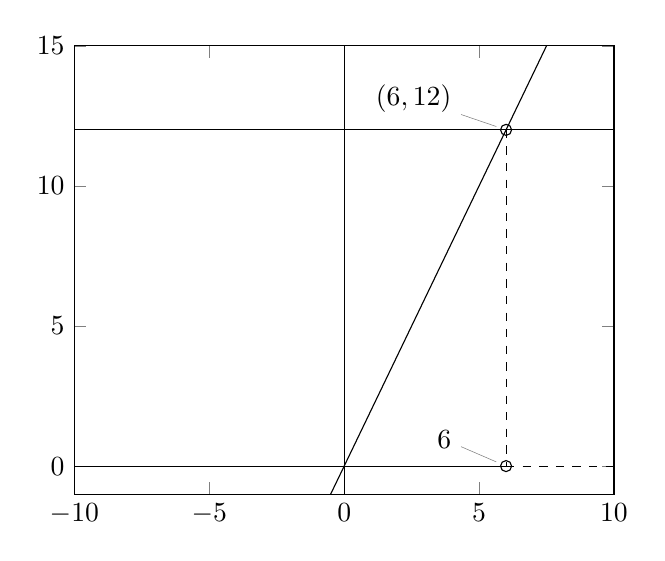
\begin{tikzpicture}
		\begin{axis}[
			xmin=-10, xmax=10,
    		ymin=-1, ymax=15,
		]
			
			\addplot[domain=-10:10] {12};
			\addplot[domain=-10:10] {2 * x};
			\addplot[only marks,mark=o] coordinates{(6,12)} node[pin=170:{$(6,12)$}]{};
			\addplot[only marks,mark=o] coordinates{(6,0)} node[pin=170:{$6$}]{};
			\addplot[dashed] coordinates{(6,12) (6,0)};
			\draw[-] (-10,0)--(6,0);
			\draw[-,dashed] (6,0)--(10,0);
			\draw[-] (0,-25)--(0,15);
		\end{axis}
	\end{tikzpicture}
\end{center}
\subsection{Solving General inequalities}
If we can put an inequality in the form $f(x) < 0$ or a variation appon that with a different relational operator,
When we graph $f(x)$ all values of $x$ that satisfy the inequality are below (or above depending on the operator)
the $x$ axis as shown below:
\begin{center}
	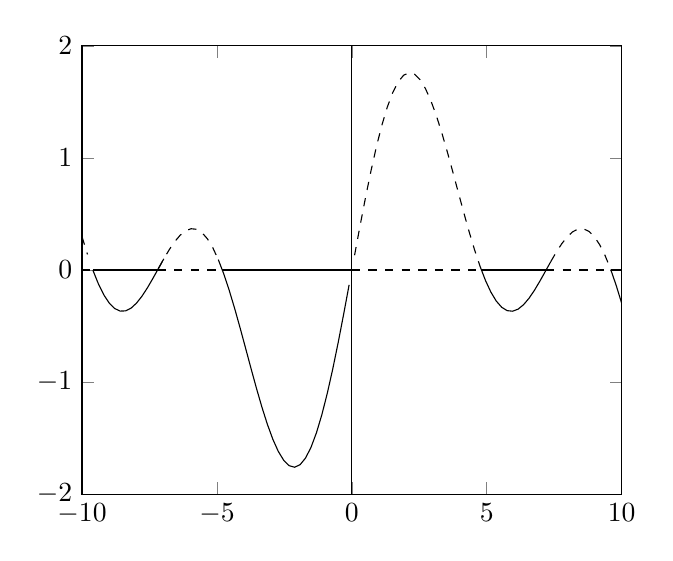
\begin{tikzpicture}
		\begin{axis}[
			xmin=-10, xmax=10,
    		ymin=-2, ymax=2,
		]
			
			\addplot[samples=100,domain=-10:10,restrict y to domain={0:2},dashed] {sin(50 * x) + sin(25 * x)};
			\addplot[samples=100,domain=-10:10,restrict y to domain={-2:0.1}] {sin(50 * x) + sin(25 * x)};

			\draw[-,dashed] (-10,0)--(-9.6,0);
			\draw[-] (-9.6,0)--(-7.2,0);
			\draw[-,dashed] (-7.2,0)--(-4.8,0);
			\draw[-] (-4.8,0)--(0,0);
			\draw[-,dashed] (0,0)--(4.8,0);
			\draw[-] (4.8,0)--(7.2,0);
			\draw[-,dashed] (7.2,0)--(9.6,0);
			\draw[-] (9.6,0)--(10,0);
			\draw[-] (0,-25)--(0,15);
		\end{axis}
	\end{tikzpicture}
\end{center}
However, there are multiple points regions where the inequality is satisfied. We can list all of them in the form $x < b$,
$x > b$ and so on.

\break

\subsection{Quadratic Inequalities}
To solve quadratic inequalities we must rearrange and find the roots just like solving any other quadratic.
For example, given the quadratic $x(x+1) < 6$ we can do the following:
\begin{equation}
	x(x+1) < 6 \Rightarrow x(x+1) - 6 < 0 \Rightarrow (x + 3)(x - 2) < 0 \Rightarrow -3 < x < 2
\end{equation}
This can be represented graphically as the following:

\begin{center}
	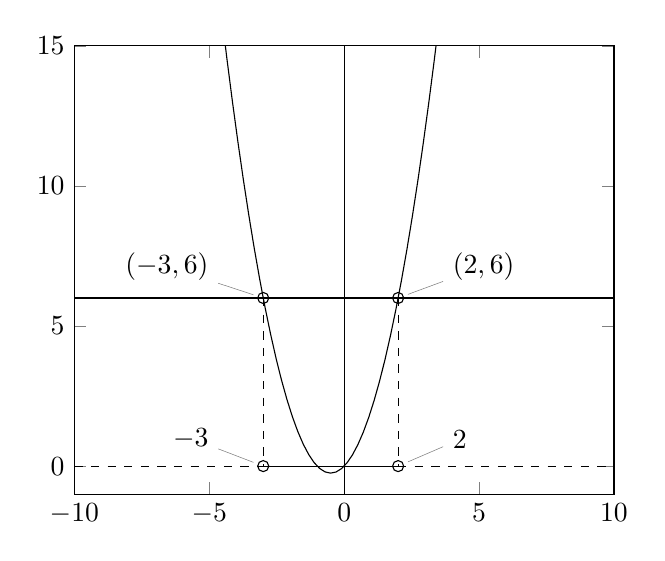
\begin{tikzpicture}
		\begin{axis}[
			xmin=-10, xmax=10,
    		ymin=-1, ymax=15,
		]
			
			\addplot[domain=-10:10] {6};
			\addplot[samples=100,domain=-10:10] {x * (x+1)};
			\addplot[only marks,mark=o] coordinates{(-3,6)} node[pin=170:{$(-3,6)$}]{};
			\addplot[only marks,mark=o] coordinates{(-3,0)} node[pin=170:{$-3$}]{};
			\addplot[only marks,mark=o] coordinates{(2,6)} node[pin=10:{$(2,6)$}]{};
			\addplot[only marks,mark=o] coordinates{(2,0)} node[pin=10:{$2$}]{};
			\addplot[dashed] coordinates{(-3,6) (-3,0)};
			\addplot[dashed] coordinates{(2,6) (2,0)};
			\draw[-,dashed] (-10,0)--(-3,0);
			\draw[-] (-3,0)--(2,0);
			\draw[-,dashed] (2,0)--(10,0);
			\draw[-] (0,-25)--(0,15);
		\end{axis}
	\end{tikzpicture}
\end{center}

\break

\subsection{Double and Triple Inequalities}
When solving double and triple inequalities it's important to remember to do everything to all sides. For example, if multiplying
by $5$ multiply all sides by $5$.
\\
Double and triple inequalities can be solved using the basic rules of algebra as shown below:
\begin{equation}
	8 < \frac{2x - 3}{5} < 10 \Rightarrow 40 < 2x - 3 < 50 \Rightarrow 43 < 2x < 53 \Rightarrow \frac{43}{2} < x < \frac{53}{2}
\end{equation}
We can also solve inequalities seperately as shown below:
\begin{gather*}
	8 < \frac{2x - 3}{5} \Rightarrow 40 < 2x - 3 \Rightarrow 43 < 2x \Rightarrow \frac{43}{2} < x \\
	\frac{2x - 3}{5} < 10 \Rightarrow 2x - 3 < 50 \Rightarrow 2x < 53 \Rightarrow x < \frac{53}{2}\\
	\text{We can then combine them together into the following:}\\
	\frac{43}{2} < x < \frac{53}{2}
\end{gather*}
Often it can be easier to solve them seperately however, it can sometimes be unclear how to combine inequalities
such as the following:
\begin{equation}
	[x < -\sqrt{2} \text{ or } x > -\sqrt{2}]\text{ and }[x < -\sqrt{6} \text{ or } x > \sqrt{6} ]
\end{equation}
Often it becomes clearer when they are sketched as shown below:

\begin{center}
	\begin{tikzpicture}
		\begin{axis}[
    		ymin=-3, ymax=3,
			ymajorticks=false
		]

		\draw[-] (-10,1)--(-2.45,1);
		\addplot[only marks,mark=o] coordinates{(-2.45,1)} node[pin=90:{$-\sqrt{6}$}]{};
		\draw[-] (10,1)--(2.45,1);
		\addplot[only marks,mark=o] coordinates{(2.45,1)} node[pin=90:{$\sqrt{6}$}]{};
		\draw[-] (-10,-1)--(-1.75,-1);
		\addplot[only marks,mark=o] coordinates{(-1.75,-1)} node[pin=-90:{$-\sqrt{3}$}]{};
		\draw[-] (10,-1)--(1.75,-1);
		\addplot[only marks,mark=o] coordinates{(1.75,-1)} node[pin=-90:{$\sqrt{3}$}]{};

		\end{axis}
	\end{tikzpicture}
\end{center}
Now we can easily see that $x < -\sqrt{6}$ or $x > \sqrt{6}$ is the solution as $x < -\sqrt{3}$ or $x > \sqrt{3}$
covers more than is wanted.

\break

\subsubsection{Triple Inequalities}
We can solve triple inequalities by first slitting up and simplifying individual inequalities.
For example, $2x - 3 < 5x + 2 < 6x + 7 < 5x + 9$ can be broken up into $x > -\frac{5}{3}$, $x > 9$ and $x > 16$.
We can then find the final inequality by plotting them as follows:

\begin{center}
	\begin{tikzpicture}
		\begin{axis}[
    		ymin=-2, ymax=2,
			ymajorticks=false
		]

		\draw[-] (-20,1)--(16,1);
		\addplot[only marks,mark=o] coordinates{(16,1)} node[pin=90:{$16$}]{};
		\draw[-] (-1.67,-1)--(20,-1);
		\addplot[only marks,mark=o] coordinates{(-1.67,-1)} node[pin=-90:{$-\frac{5}{3}$}]{};
		\draw[-] (9,0)--(20,0);
		\addplot[only marks,mark=o] coordinates{(9,0)} node[pin=-90:{$9$}]{};

		\draw[-,dashed] (9,-5)--(9,5);
		\draw[-,dashed] (16,-5)--(16,5);

		\end{axis}
	\end{tikzpicture}
\end{center}
From this diagram we can clearly see that the only place where all of these inequalities are true is between $9$ and $16$
therefore $9 < x < 16$.

\pgfplotsset{IneqStyleGtr/.style = {%
   decoration={border,segment length=1mm, amplitude=5mm,angle=-90},
          postaction={decorate,draw},
          thick,blue!50!white, draw opacity=0.5
  }
}

\pgfplotsset{IneqStyleLess/.style = {%
   decoration={border,segment length=1mm, amplitude=5mm,angle=90},
              postaction={decorate,draw},
              thick,blue!50!white, draw opacity=0.5
  }
}

\break

\subsection{Representing Inequalities Graphically}
When representing inequalities graphically it's important to remember to use a doted line for $<$ and $>$
and a solid line for $\leq$ and $\geq$.
\\\\
Below shows some linear Inequalities drawn on a graph:
\begin{center}
	\begin{tikzpicture}
		\begin{axis}[
			xmin=-5, xmax=5,
    		ymin=-2, ymax=6,	
		]

		\addplot[IneqStyleGtr,dashed,thin] {x + 2};
		\addplot[dashed] {x + 2};

		\addplot[IneqStyleLess,thin] {(8 - x) / 2};
		\addplot[] {(8 - x) / 2};

		\addplot[] coordinates{(2,3.2)} node[label=0:{$2y + x \leq 8$}]{};
		\addplot[] coordinates{(-2,0)} node[label=0:{$y > x + 2$}]{};

		\end{axis}
	\end{tikzpicture}
\end{center}
Similarly we can draw quadratic inequalities as shown below:

\begin{center}
	\begin{tikzpicture}
		\begin{axis}[
			xmin=-5, xmax=5,
    		ymin=-5, ymax=6,	
		]

		\addplot[IneqStyleGtr,dashed,thin] {x^2 + 1};
		\addplot[dashed] {x^2 + 1};

		\addplot[IneqStyleLess,thin] {x^2 - 4};
		\addplot[] {x^2 - 4};

		\addplot[] coordinates{(-1.6,4)} node[label=0:{$y > x^2 + 1$}]{};
		\addplot[] coordinates{(-3.5,-4)} node[label=0:{$y \leq x ^2 - 4$}]{};

		\end{axis}
	\end{tikzpicture}
\end{center}

\break

\subsection{Identifying Regions Graphically}
When identifying regions, in most cases, we need to draw multiple inequalities. Given the following inequalities
we can construct the following graph:
\begin{gather*}
	x + y < 12 \\
	x \geq 0 \\
	y \geq 0
\end{gather*}

\begin{center}
	\begin{tikzpicture}
		\begin{axis}[
			xmin=-5, xmax=15,
    		ymin=-5, ymax=15,	
		]

		\addplot[IneqStyleLess,dashed,domain=-5:15,thin] {12 - x};
		\addplot[dashed,domain=-5:15] {12 - x};

		\addplot[IneqStyleGtr,domain=-5:15,thin] {0};
		\addplot[domain=-5:15] {0};
		\addplot[IneqStyleGtr,thin] coordinates{(0, 15) (0, -15)};
		\addplot[] coordinates{(0, -15) (0, 15)};

		\addplot[] coordinates{(2,4)} node[label=0:{$F.R.$}]{};

		\end{axis}
	\end{tikzpicture}
\end{center}
Note: In an exam, unless specified, do not shade the region.

\section{Graphs}

\subsection{Cubic Graphs}
Cubic graphs are graphs made from 3rd degree polynomials ($ax^3 + bx^2 + cx + d$). Cubic graphs can be drawn by calculating
points on the graph as shown below for the simplest cubic graph $x^3$:

\begin{center}
	\begin{tabular}{ | c | r | r | r | c | c | c | r | }
		\hline
		$x$ & $-3$ & $-2$ & $-1$ & $0$ & $1$ & $2$ & $3$\\ \hline
		$y=x^3$ &$-27$ & $-8$ & $-1$ & $0$ & $1$ & $8$ & $27$\\
		\hline
	\end{tabular}
\end{center}

\begin{center}
	\begin{tikzpicture}
		\begin{axis}[
			xmin=-5, xmax=5,
    		ymin=-30, ymax=30,
			axis lines=middle
		]
			\addplot[] {x^3};
			\addplot[only marks,mark=o] coordinates{(-3,-27) (-2,-8) (-1,-1) (0,0) (1,1) (2,8) (3,27)};
			\legend{$y=x^3$}
		\end{axis}
	\end{tikzpicture}
\end{center}

\subsection{Sketching Polynomials}
We can sketch polynomials in the form $y=(x + a_1)(x + a_2)(x+a_3)\cdots(x+a_n)$ by simply marking all of the $-a$s
as the roots and the product of all the $a$s as the $y$ intercept. For example, the following shows the graph
of the quartic equation $y=(x-3)(x+1)(x+2)(x+3)$:
\begin{center}
	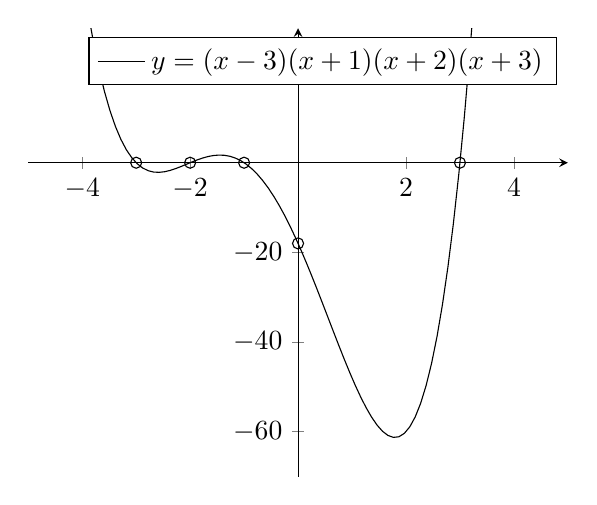
\begin{tikzpicture}
		\begin{axis}[
			xmin=-5, xmax=5,
    		ymin=-70, ymax=30,
			axis lines=middle
		]
			\addplot[samples=100,domain=-5:5] {(x-3) * (x+1) * (x+2) * (x+3)};
			\addplot[only marks,mark=o] coordinates{(-3,0) (-2,0) (-1,0) (3,0) (0,-18)};
			\legend{$y=(x-3)(x+1)(x+2)(x+3)$}
		\end{axis}
	\end{tikzpicture}
\end{center}

\section{Graph Transformations}
\subsection{Vertical Scale}
In order to strech a graph $f(x)$ on the $y$ axis by the coefficient $a$. We multiply $f(x)$ by $a$.
This can be represented as follows:
\begin{equation}
	y = af(x)
\end{equation}

\subsection{Horisontal Scale}
In order to strech a graph $f(x)$ on the $x$ axis by the coefficient $a$. We divide $x$ by $a$.
This can be represented as follows:
\begin{equation}
	y = f\left(\frac{x}{a}\right)
\end{equation}
\subsection{Vertical Translation}
In order to translate a graph $f(x)$ on the $y$ axis by $a$. We add $a$ to $f(x)$. This can be
represented as follows:

\begin{equation}
	y = f(x) + a
\end{equation}
\subsection{Horisontal Translation}
In order to translate a graph $f(x)$ on the $x$ axis by $a$. We subtract $a$ from $x$. This can be
represented as follows:

\begin{equation}
	y = f(x - a)
\end{equation}
Note: Mirroring is a special case of stretching where the coefficient is $-1$.

\end{document}
